\tikzset{>=latex} % for LaTeX arrow head

\colorlet{Ecol}{orange!90!black}
\colorlet{EcolFL}{orange!80!black}
\colorlet{veccol}{green!45!black}
\colorlet{EFcol}{red!60!black}
\tikzstyle{charged}=[top color=blue!20,bottom color=blue!40,shading angle=10]
\tikzstyle{darkcharged}=[very thin,top color=blue!60,bottom color=blue!80,shading angle=10]
\tikzstyle{charge+}=[very thin,top color=red!80,bottom color=red!80!black,shading angle=-5]
\tikzstyle{charge-}=[very thin,top color=blue!50,bottom color=blue!70!white!90!black,shading angle=10]
\tikzstyle{gauss surf}=[green!80!black,top color=green!2,bottom color=green!80!black!70,shading angle=5,fill opacity=0.6]
\tikzstyle{gauss lid}=[gauss surf,middle color=green!80!black!20,shading angle=40,fill opacity=0.6]
\tikzstyle{gauss line}=[green!80!black]
\tikzstyle{gauss dashed line}=[green!60!black!80,dashed,line width=0.2]
\tikzstyle{metal}=[top color=black!5,bottom color=black!15,shading angle=30]
\tikzstyle{vector}=[->,thick,veccol]
\tikzstyle{normalvec}=[->,thick,blue!80!black!80]
\tikzstyle{EField}=[->,thick,Ecol]
\tikzstyle{EField dashed}=[dashed,Ecol,line width=0.6]
\tikzset{
  EFieldLine/.style={thick,EcolFL,decoration={markings,
                     mark=at position #1 with {\arrow{latex}}},
                     postaction={decorate}},
  EFieldLine/.default=0.5}
\tikzstyle{measure}=[fill=white,midway,outer sep=2]

% PLANE field with electric field


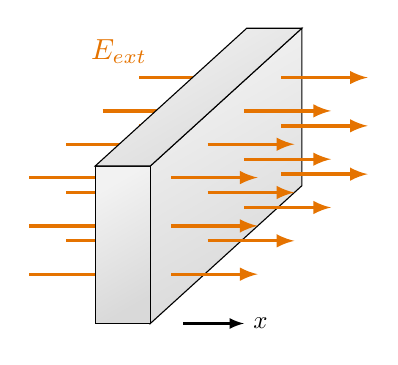
\begin{tikzpicture}[x={(1.0cm,0)},y={(0.55cm,0.5cm)},z={(0,1.0cm)}]
  \def\H{2.0}
  \def\W{0.7}
  \def\L{3.5}
  \def\Ny{5}
  \def\Nz{4}
  \def\NEy{4}
  \def\NEz{3}
  \def\oEy{0.08*\W}
  \def\oEz{0.04*\H}
  \def\E{1.1}
  
  % ELECTRIC FIELD back
  \foreach \i [evaluate={\y=\oEy+(\i-0.5)*(\L-2*\oEy)/\NEy;}] in {1,...,\NEy}{
    \foreach \j [evaluate={\z=\oEz+(\j-0.5)*(\H-2*\oEz)/\NEz;}] in {1,...,\NEz}{
      \draw[EField,very thick] (-\E,\y,\z) --++ (\E,0,0);
    }
  }
  
  % AXIS
  \draw[->,thick] (1.6*\W,0,0) --++ (1.1*\W,0,0) node[right,scale=0.9] {$x$};
  
  % PLANE
  \draw[metal]
    (\W,0,0) --++ (0,\L,0) --++ (0,0,\H) --++ (0,-\L,0) -- cycle;
  \draw[metal]
    (0,0,0) --++ (\W,0,0) --++ (0,0,\H) --++ (-\W,0,0) -- cycle;
  \draw[metal]
    (0,0,\H) --++ (\W,0,0) --++ (0,\L,0) --++ (-\W,0,0) -- cycle;
  
  % ELECTRIC FIELD front
  \foreach \i [evaluate={\y=\oEy+(\i-0.5)*(\L-2*\oEy)/\NEy;}] in {1,...,\NEy}{
    \foreach \j [evaluate={\z=\oEz+(\j-0.5)*(\H-2*\oEz)/\NEz;}] in {1,...,\NEz}{
      \draw[EField,very thick] (\W,\y,\z) --++ (\E,0,0);
    }
  }
  %\node[Ecol,scale=1.05] at (\W+\E,0.9*\L,0.93*\H) {$\vb{E}_\text{ext}$};
  \node[Ecol,scale=1.05] at (-1.3*\E,0.9*\L,0.94*\H) {$\vb{E}_\text{ext}$};
  %\node[Ecol,scale=1.05] at (\W+1.3*\E,0.2*\L,0.1*\H) {$\vb{E}_\text{ext}$};
  
\end{tikzpicture}
